\documentclass[a4paper, UTF8]{ctexart}
\usepackage{ctex}
\usepackage{amsmath}
\usepackage{amsthm}
\usepackage{multirow}
\usepackage{amssymb}
\usepackage{graphicx}
\usepackage{geometry}
\usepackage{bm}
\usepackage{subfigure}
\usepackage{float}
\usepackage{mathrsfs}
\renewcommand\thesection{\arabic{section}}
\newtheorem*{exercise}{\textbf{习题}}
\newtheorem*{theorem}{Theorem}
\title{Manifole Learning Homework 7}
\date{\today}
\author{安捷 1601210097}
\begin{document}
\maketitle
  \begin{exercise}[103-108]
  	我调用sklearn软件包分别使用上述作业要求中的算法对所有类别的人脸图像进行降维,结果如下:\\
  	\begin{figure}[htbp!]
  		\centering
  		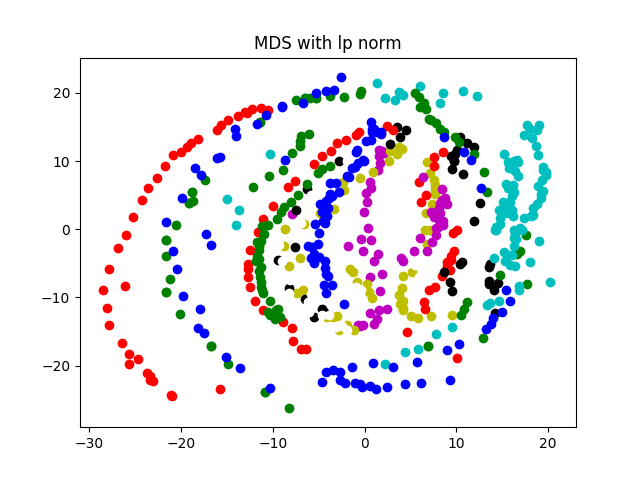
\includegraphics[width = \textwidth]{hw7_fig1.png}
  	\end{figure}
  	\clearpage
  	\begin{figure}[htbp!]
  		\centering
  		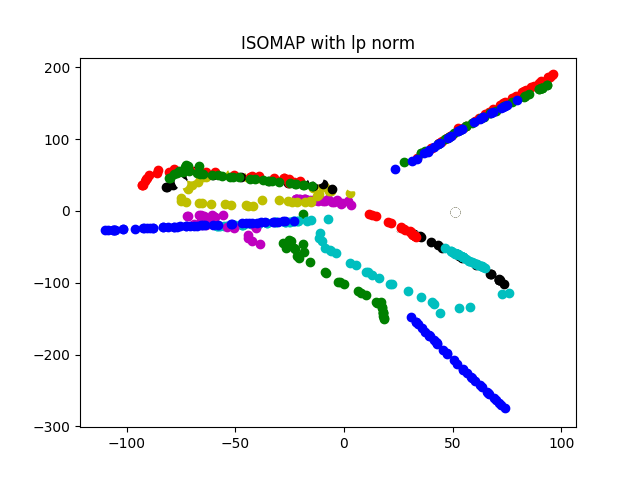
\includegraphics[width = \textwidth]{hw7_fig2.png}
  	\end{figure}
  	\clearpage
  	\begin{figure}[htbp!]
  		\centering
  		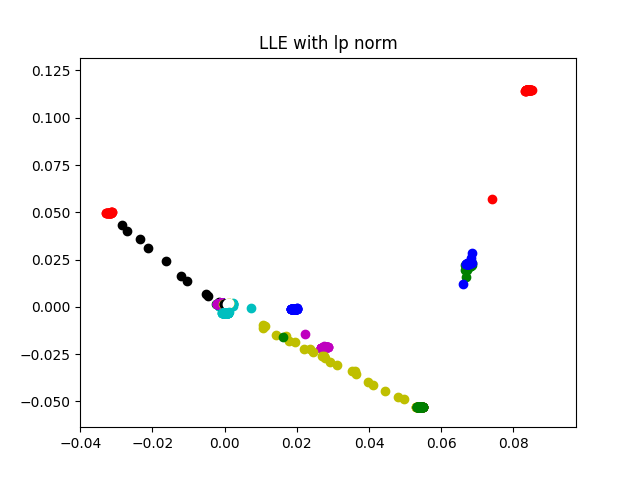
\includegraphics[width = \textwidth]{hw7_fig3.png}
  	\end{figure}
  	\clearpage
  	\begin{figure}[htbp!]
  		\centering
  		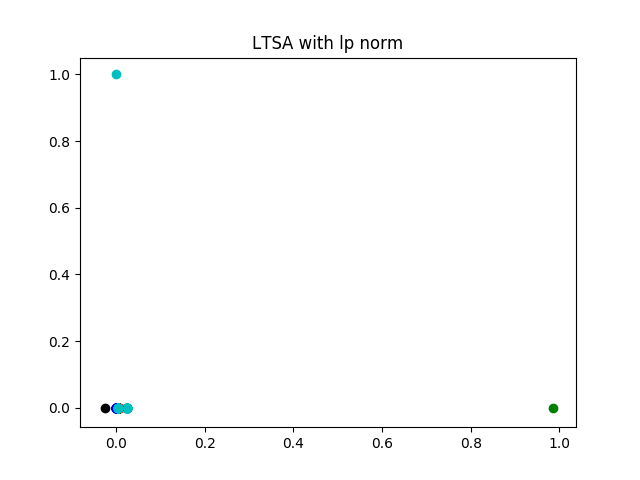
\includegraphics[width = \textwidth]{hw7_fig4.png}
  	\end{figure}
  	\clearpage
  	\begin{figure}[htbp!]
  		\centering
  		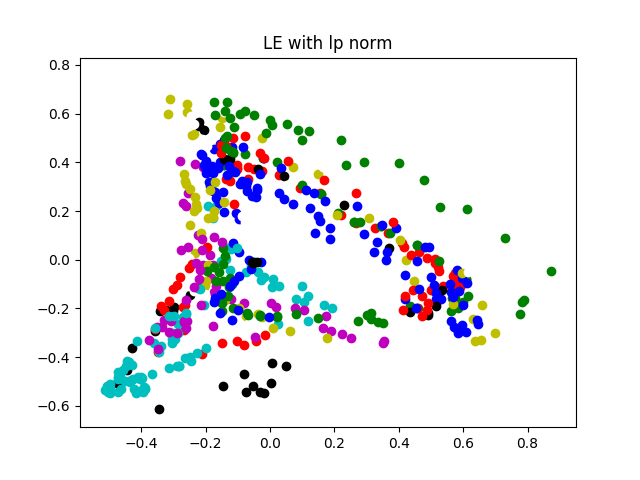
\includegraphics[width = \textwidth]{hw7_fig5.png}
  	\end{figure}
  	\clearpage
  	从图中明显可以看出,LLE与ISOMAP对于人脸图像的分类降维效果较好,在降至2维的情况下对图像有很好的表现效果。
  \end{exercise}
\end{document}